\documentclass[tikz,border=10pt]{standalone}
\usepackage[T1]{fontenc}
\usepackage{helvet}
\renewcommand{\familydefault}{\sfdefault}
\usepackage{tikz}
\usetikzlibrary{arrows.meta,positioning,shapes.multipart,shapes.geometric,fit,backgrounds,calc,shadows}

\definecolor{navy}{HTML}{1F3A5F}
\definecolor{teal}{HTML}{0C6B58}
\definecolor{amber}{HTML}{D9822B}
\definecolor{crimson}{HTML}{B42318}
\definecolor{violet}{HTML}{6B21A8}
\definecolor{sky}{HTML}{2186EB}
\definecolor{slate}{HTML}{486581}
\definecolor{mist}{HTML}{F0F4F8}
\definecolor{line}{HTML}{9FB3C8}

\tikzset{
  >={Stealth[length=2.6mm]},
  box/.style={draw=navy, very thick, rounded corners=3pt, fill=white, align=center,
    inner sep=5pt, font=\small, minimum height=9mm},
  softbox/.style={box, draw=slate, thick, fill=mist},
  layer/.style={draw=line, dashed, rounded corners=6pt, inner sep=7pt},
  layertitle/.style={font=\bfseries\small, text=slate, anchor=north west},
  flow/.style={->, thick, draw=navy},
  dflow/.style={->, thick, draw=slate, dashed},
  lbl/.style={font=\scriptsize, text=slate, fill=white, inner sep=1.5pt},
  umlclass/.style={draw=navy, thick, fill=white, rectangle split, rectangle split parts=3,
    rectangle split part fill={navy!12,white,white}, align=left, font=\scriptsize,
    inner sep=3pt, text width=#1},
  umlclass/.default=38mm,
}

\tikzset{
  stage/.style={box, minimum width=4.6cm, font=\scriptsize},
  det/.style={box, draw=violet, minimum width=3.0cm, font=\scriptsize, minimum height=1.6cm, text width=2.8cm},
  dec/.style={diamond, aspect=2.2, draw=amber, very thick, fill=white, align=center, font=\scriptsize, inner sep=1pt},
  term/.style={box, rounded corners=9pt, draw=teal, font=\scriptsize},
}
\begin{document}
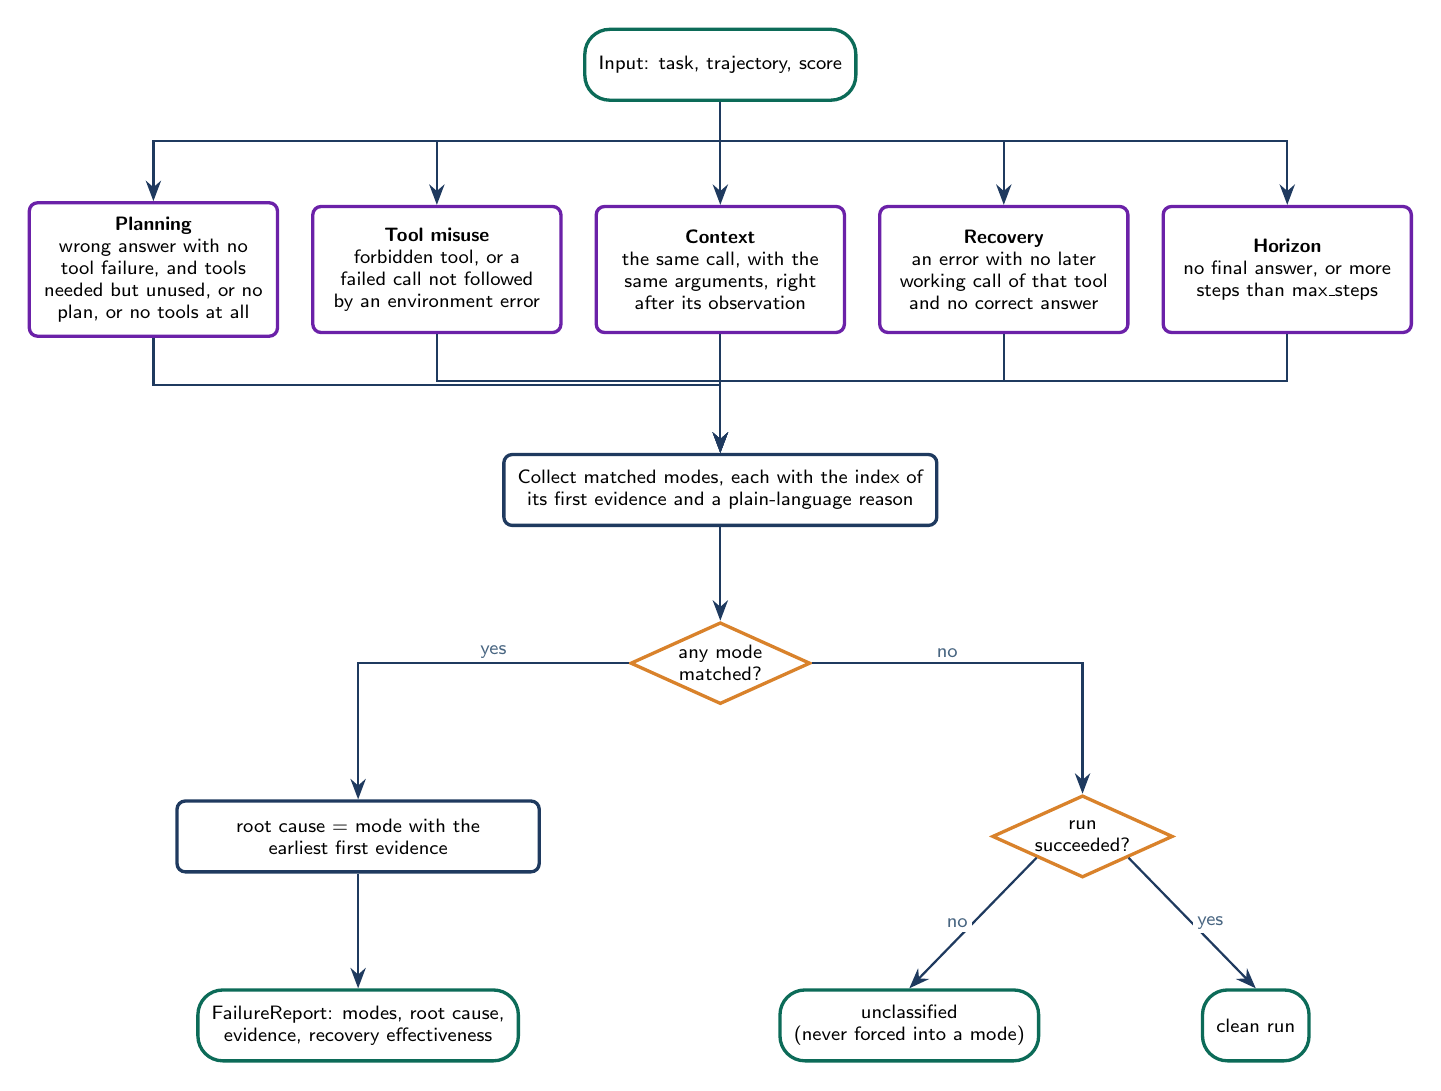
\begin{tikzpicture}[x=1cm,y=1cm]
  \node[term] (in) at (0,0) {Input: task, trajectory, score};
  \node[det] (d1) at (-7.2,-2.6) {\textbf{Planning}\\wrong answer with no tool failure, and tools needed but unused, or no plan, or no tools at all};
  \node[det] (d2) at (-3.6,-2.6) {\textbf{Tool misuse}\\forbidden tool, or a failed call not followed by an environment error};
  \node[det] (d3) at (0,-2.6) {\textbf{Context}\\the same call, with the same arguments, right after its observation};
  \node[det] (d4) at (3.6,-2.6) {\textbf{Recovery}\\an error with no later working call of that tool and no correct answer};
  \node[det] (d5) at (7.2,-2.6) {\textbf{Horizon}\\no final answer, or more steps than max\_steps};
  \foreach \d in {d1,d2,d3,d4,d5} { \draw[flow] (in.south) -- ++(0,-0.5) -| (\d.north); }

  \node[stage] (collect) at (0,-5.4) {Collect matched modes, each with the index of\\its first evidence and a plain-language reason};
  \foreach \d in {d1,d2,d3,d4,d5} { \draw[flow] (\d.south) -- ++(0,-0.6) -| (collect.north); }

  \node[dec] (any) at (0,-7.6) {any mode\\matched?};
  \draw[flow] (collect) -- (any);
  \node[stage] (root) at (-4.6,-9.8) {root cause = mode with the\\earliest first evidence};
  \node[dec] (ok) at (4.6,-9.8) {run\\succeeded?};
  \draw[flow] (any.west) -| node[lbl, pos=0.25, above] {yes} (root.north);
  \draw[flow] (any.east) -| node[lbl, pos=0.25, above] {no} (ok.north);
  \node[term] (unc) at (2.4,-12.2) {unclassified\\(never forced into a mode)};
  \node[term] (clean) at (6.8,-12.2) {clean run};
  \draw[flow] (ok.south west) -- node[lbl, left] {no} (unc.north);
  \draw[flow] (ok.south east) -- node[lbl, right] {yes} (clean.north);
  \node[term] (out) at (-4.6,-12.2) {FailureReport: modes, root cause,\\evidence, recovery effectiveness};
  \draw[flow] (root) -- (out);
\end{tikzpicture}
\end{document}
